\documentclass[1p]{elsarticle_modified}
%\bibliographystyle{elsarticle-num}

%\usepackage[colorlinks]{hyperref}
%\usepackage{abbrmath_seonhwa} %\Abb, \Ascr, \Acal ,\Abf, \Afrak
\usepackage{amsfonts}
\usepackage{amssymb}
\usepackage{amsmath}
\usepackage{amsthm}
\usepackage{scalefnt}
\usepackage{amsbsy}
\usepackage{kotex}
\usepackage{caption}
\usepackage{subfig}
\usepackage{color}
\usepackage{graphicx}
\usepackage{xcolor} %% white, black, red, green, blue, cyan, magenta, yellow
\usepackage{float}
\usepackage{setspace}
\usepackage{hyperref}

\usepackage{tikz}
\usetikzlibrary{arrows}

\usepackage{multirow}
\usepackage{array} % fixed length table
\usepackage{hhline}

%%%%%%%%%%%%%%%%%%%%%
\makeatletter
\renewcommand*\env@matrix[1][\arraystretch]{%
	\edef\arraystretch{#1}%
	\hskip -\arraycolsep
	\let\@ifnextchar\new@ifnextchar
	\array{*\c@MaxMatrixCols c}}
\makeatother %https://tex.stackexchange.com/questions/14071/how-can-i-increase-the-line-spacing-in-a-matrix
%%%%%%%%%%%%%%%

\usepackage[normalem]{ulem}

\newcommand{\msout}[1]{\ifmmode\text{\sout{\ensuremath{#1}}}\else\sout{#1}\fi}
%SOURCE: \msout is \stkout macro in https://tex.stackexchange.com/questions/20609/strikeout-in-math-mode

\newcommand{\cancel}[1]{
	\ifmmode
	{\color{red}\msout{#1}}
	\else
	{\color{red}\sout{#1}}
	\fi
}

\newcommand{\add}[1]{
	{\color{blue}\uwave{#1}}
}

\newcommand{\replace}[2]{
	\ifmmode
	{\color{red}\msout{#1}}{\color{blue}\uwave{#2}}
	\else
	{\color{red}\sout{#1}}{\color{blue}\uwave{#2}}
	\fi
}

\newcommand{\Sol}{\mathcal{S}} %segment
\newcommand{\D}{D} %diagram
\newcommand{\A}{\mathcal{A}} %arc


%%%%%%%%%%%%%%%%%%%%%%%%%%%%%5 test

\def\sl{\operatorname{\textup{SL}}(2,\Cbb)}
\def\psl{\operatorname{\textup{PSL}}(2,\Cbb)}
\def\quan{\mkern 1mu \triangleright \mkern 1mu}

\theoremstyle{definition}
\newtheorem{thm}{Theorem}[section]
\newtheorem{prop}[thm]{Proposition}
\newtheorem{lem}[thm]{Lemma}
\newtheorem{ques}[thm]{Question}
\newtheorem{cor}[thm]{Corollary}
\newtheorem{defn}[thm]{Definition}
\newtheorem{exam}[thm]{Example}
\newtheorem{rmk}[thm]{Remark}
\newtheorem{alg}[thm]{Algorithm}

\newcommand{\I}{\sqrt{-1}}
\begin{document}

%\begin{frontmatter}
%
%\title{Boundary parabolic representations of knots up to 8 crossings}
%
%%% Group authors per affiliation:
%\author{Yunhi Cho} 
%\address{Department of Mathematics, University of Seoul, Seoul, Korea}
%\ead{yhcho@uos.ac.kr}
%
%
%\author{Seonhwa Kim} %\fnref{s_kim}}
%\address{Center for Geometry and Physics, Institute for Basic Science, Pohang, 37673, Korea}
%\ead{ryeona17@ibs.re.kr}
%
%\author{Hyuk Kim}
%\address{Department of Mathematical Sciences, Seoul National University, Seoul 08826, Korea}
%\ead{hyukkim@snu.ac.kr}
%
%\author{Seokbeom Yoon}
%\address{Department of Mathematical Sciences, Seoul National University, Seoul, 08826,  Korea}
%\ead{sbyoon15@snu.ac.kr}
%
%\begin{abstract}
%We find all boundary parabolic representation of knots up to 8 crossings.
%
%\end{abstract}
%\begin{keyword}
%    \MSC[2010] 57M25 
%\end{keyword}
%
%\end{frontmatter}

%\linenumbers
%\tableofcontents
%
\newcommand\colored[1]{\textcolor{white}{\rule[-0.35ex]{0.8em}{1.4ex}}\kern-0.8em\color{red} #1}%
%\newcommand\colored[1]{\textcolor{white}{ #1}\kern-2.17ex	\textcolor{white}{ #1}\kern-1.81ex	\textcolor{white}{ #1}\kern-2.15ex\color{red}#1	}

{\Large $\underline{12n_{0226}~(K12n_{0226})}$}

\setlength{\tabcolsep}{10pt}
\renewcommand{\arraystretch}{1.6}
\vspace{1cm}\begin{tabular}{m{100pt}>{\centering\arraybackslash}m{274pt}}
\multirow{5}{120pt}{
	\centering
	\includegraphics[width=112pt]{../../../GIT/diagram.site/Diagrams/png/2315_12n_0226.png}\\
\ \ \ A knot diagram\footnotemark}&
\allowdisplaybreaks
\textbf{Linearized knot diagam} \\
\cline{2-2}
 &
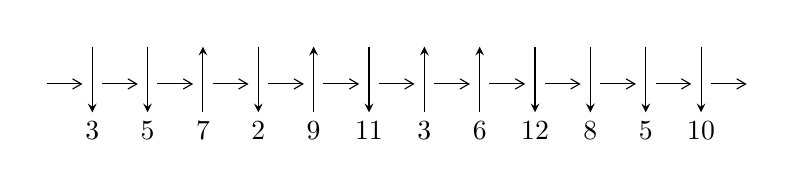
\begin{tikzpicture}[x=20pt, y=17pt]
	% nodes
	\node (C0) at (0, 0) {};
	\node (C1) at (1, 0) {};
	\node (C1U) at (1, +1) {};
	\node (C1D) at (1, -1) {3};

	\node (C2) at (2, 0) {};
	\node (C2U) at (2, +1) {};
	\node (C2D) at (2, -1) {5};

	\node (C3) at (3, 0) {};
	\node (C3U) at (3, +1) {};
	\node (C3D) at (3, -1) {7};

	\node (C4) at (4, 0) {};
	\node (C4U) at (4, +1) {};
	\node (C4D) at (4, -1) {2};

	\node (C5) at (5, 0) {};
	\node (C5U) at (5, +1) {};
	\node (C5D) at (5, -1) {9};

	\node (C6) at (6, 0) {};
	\node (C6U) at (6, +1) {};
	\node (C6D) at (6, -1) {11};

	\node (C7) at (7, 0) {};
	\node (C7U) at (7, +1) {};
	\node (C7D) at (7, -1) {3};

	\node (C8) at (8, 0) {};
	\node (C8U) at (8, +1) {};
	\node (C8D) at (8, -1) {6};

	\node (C9) at (9, 0) {};
	\node (C9U) at (9, +1) {};
	\node (C9D) at (9, -1) {12};

	\node (C10) at (10, 0) {};
	\node (C10U) at (10, +1) {};
	\node (C10D) at (10, -1) {8};

	\node (C11) at (11, 0) {};
	\node (C11U) at (11, +1) {};
	\node (C11D) at (11, -1) {5};

	\node (C12) at (12, 0) {};
	\node (C12U) at (12, +1) {};
	\node (C12D) at (12, -1) {10};
	\node (C13) at (13, 0) {};

	% arrows
	\draw[->,>={angle 60}]
	(C0) edge (C1) (C1) edge (C2) (C2) edge (C3) (C3) edge (C4) (C4) edge (C5) (C5) edge (C6) (C6) edge (C7) (C7) edge (C8) (C8) edge (C9) (C9) edge (C10) (C10) edge (C11) (C11) edge (C12) (C12) edge (C13) ;	\draw[->,>=stealth]
	(C1U) edge (C1D) (C2U) edge (C2D) (C3D) edge (C3U) (C4U) edge (C4D) (C5D) edge (C5U) (C6U) edge (C6D) (C7D) edge (C7U) (C8D) edge (C8U) (C9U) edge (C9D) (C10U) edge (C10D) (C11U) edge (C11D) (C12U) edge (C12D) ;
	\end{tikzpicture} \\
\hhline{~~} \\& 
\textbf{Solving Sequence} \\ \cline{2-2} 
 &
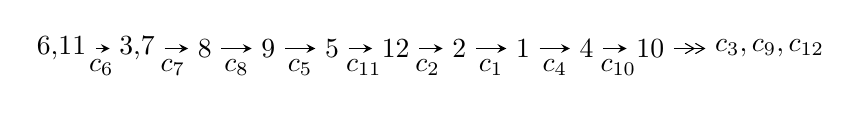
\begin{tikzpicture}[x=23pt, y=7pt]
	% node
	\node (A0) at (-1/8, 0) {6,11};
	\node (A1) at (17/16, 0) {3,7};
	\node (A2) at (17/8, 0) {8};
	\node (A3) at (25/8, 0) {9};
	\node (A4) at (33/8, 0) {5};
	\node (A5) at (41/8, 0) {12};
	\node (A6) at (49/8, 0) {2};
	\node (A7) at (57/8, 0) {1};
	\node (A8) at (65/8, 0) {4};
	\node (A9) at (73/8, 0) {10};
	\node (C1) at (1/2, -1) {$c_{6}$};
	\node (C2) at (13/8, -1) {$c_{7}$};
	\node (C3) at (21/8, -1) {$c_{8}$};
	\node (C4) at (29/8, -1) {$c_{5}$};
	\node (C5) at (37/8, -1) {$c_{11}$};
	\node (C6) at (45/8, -1) {$c_{2}$};
	\node (C7) at (53/8, -1) {$c_{1}$};
	\node (C8) at (61/8, -1) {$c_{4}$};
	\node (C9) at (69/8, -1) {$c_{10}$};
	\node (A10) at (11, 0) {$c_{3},c_{9},c_{12}$};

	% edge
	\draw[->,>=stealth]	
	(A0) edge (A1) (A1) edge (A2) (A2) edge (A3) (A3) edge (A4) (A4) edge (A5) (A5) edge (A6) (A6) edge (A7) (A7) edge (A8) (A8) edge (A9) ;
	\draw[->>,>={angle 60}]	
	(A9) edge (A10);
\end{tikzpicture} \\ 

\end{tabular} \\

\footnotetext{
The image of knot diagram is generated by the software ``\textbf{Draw programme}" developed by Andrew Bartholomew(\url{http://www.layer8.co.uk/maths/draw/index.htm\#Running-draw}), where we modified some parts for our purpose(\url{https://github.com/CATsTAILs/LinksPainter}).
}\phantom \\ \newline 
\centering \textbf{Ideals for irreducible components\footnotemark of $X_{\text{par}}$} 
 
\begin{align*}
I^u_{1}&=\langle 
1.38993\times10^{213} u^{52}-3.85126\times10^{213} u^{51}+\cdots+8.47410\times10^{215} b+8.97607\times10^{216},\\
\phantom{I^u_{1}}&\phantom{= \langle  }2.88140\times10^{215} u^{52}-8.01190\times10^{215} u^{51}+\cdots+4.57601\times10^{217} a+1.91823\times10^{219},\\
\phantom{I^u_{1}}&\phantom{= \langle  }u^{53}-2 u^{52}+\cdots+22464 u+5184\rangle \\
I^u_{2}&=\langle 
u^8+u^6+2 u^4+u^2+b+u,\;u^8+u^7+3 u^6+u^5+4 u^4+u^3+4 u^2+a+2,\\
\phantom{I^u_{2}}&\phantom{= \langle  }u^9+u^8+2 u^7+u^6+3 u^5+u^4+2 u^3+u-1\rangle \\
\\
I^v_{1}&=\langle 
a,\;18315 v^5+20514 v^4+76517 v^3+68962 v^2+11867 b-4895 v+9310,\\
\phantom{I^v_{1}}&\phantom{= \langle  }9 v^6+3 v^5+38 v^4+6 v^3+7 v^2+3 v+1\rangle \\
\end{align*}
\raggedright * 3 irreducible components of $\dim_{\mathbb{C}}=0$, with total 68 representations.\\
\footnotetext{All coefficients of polynomials are rational numbers. But the coefficients are sometimes approximated in decimal forms when there is not enough margin.}
\newpage
\renewcommand{\arraystretch}{1}
\centering \section*{I. $I^u_{1}= \langle 1.39\times10^{213} u^{52}-3.85\times10^{213} u^{51}+\cdots+8.47\times10^{215} b+8.98\times10^{216},\;2.88\times10^{215} u^{52}-8.01\times10^{215} u^{51}+\cdots+4.58\times10^{217} a+1.92\times10^{219},\;u^{53}-2 u^{52}+\cdots+22464 u+5184 \rangle$}
\flushleft \textbf{(i) Arc colorings}\\
\begin{tabular}{m{7pt} m{180pt} m{7pt} m{180pt} }
\flushright $a_{6}=$&$\begin{pmatrix}1\\0\end{pmatrix}$ \\
\flushright $a_{11}=$&$\begin{pmatrix}0\\u\end{pmatrix}$ \\
\flushright $a_{3}=$&$\begin{pmatrix}-0.00629675 u^{52}+0.0175085 u^{51}+\cdots-128.153 u-41.9191\\-0.00164021 u^{52}+0.00454474 u^{51}+\cdots-31.1195 u-10.5924\end{pmatrix}$ \\
\flushright $a_{7}=$&$\begin{pmatrix}1\\u^2\end{pmatrix}$ \\
\flushright $a_{8}=$&$\begin{pmatrix}0.00570365 u^{52}-0.0158936 u^{51}+\cdots+113.481 u+37.6349\\0.00300075 u^{52}-0.00832795 u^{51}+\cdots+62.3538 u+20.6068\end{pmatrix}$ \\
\flushright $a_{9}=$&$\begin{pmatrix}0.00870440 u^{52}-0.0242216 u^{51}+\cdots+175.834 u+58.2417\\0.00300075 u^{52}-0.00832795 u^{51}+\cdots+62.3538 u+20.6068\end{pmatrix}$ \\
\flushright $a_{5}=$&$\begin{pmatrix}0.000384770 u^{52}-0.000892176 u^{51}+\cdots+10.3952 u+5.00364\\0.00146358 u^{52}-0.00397329 u^{51}+\cdots+32.4577 u+10.6141\end{pmatrix}$ \\
\flushright $a_{12}=$&$\begin{pmatrix}0.00264793 u^{52}-0.00764690 u^{51}+\cdots+49.3301 u+15.6401\\-0.00203270 u^{52}+0.00553763 u^{51}+\cdots-41.9729 u-14.2915\end{pmatrix}$ \\
\flushright $a_{2}=$&$\begin{pmatrix}-0.00349732 u^{52}+0.00965215 u^{51}+\cdots-71.0018 u-24.3376\\-0.000464535 u^{52}+0.00120085 u^{51}+\cdots-9.87081 u-3.79816\end{pmatrix}$ \\
\flushright $a_{1}=$&$\begin{pmatrix}0.000762957 u^{52}-0.00212328 u^{51}+\cdots+15.5695 u+6.49566\\0.00230398 u^{52}-0.00638244 u^{51}+\cdots+45.5648 u+14.7106\end{pmatrix}$ \\
\flushright $a_{4}=$&$\begin{pmatrix}-0.00418756 u^{52}+0.0117419 u^{51}+\cdots-81.5052 u-27.0323\\-0.000471548 u^{52}+0.00132482 u^{51}+\cdots-7.27553 u-2.56665\end{pmatrix}$ \\
\flushright $a_{10}=$&$\begin{pmatrix}0.00778197 u^{52}-0.0219456 u^{51}+\cdots+153.438 u+50.5587\\0.000923497 u^{52}-0.00264094 u^{51}+\cdots+18.6239 u+5.59256\end{pmatrix}$\\&\end{tabular}
\flushleft \textbf{(ii) Obstruction class $= -1$}\\~\\
\flushleft \textbf{(iii) Cusp Shapes $= 0.0103737 u^{52}-0.0284322 u^{51}+\cdots+214.510 u+70.9728$}\\~\\
\newpage\renewcommand{\arraystretch}{1}
\flushleft \textbf{(iv) u-Polynomials at the component}\newline \\
\begin{tabular}{m{50pt}|m{274pt}}
Crossings & \hspace{64pt}u-Polynomials at each crossing \\
\hline $$\begin{aligned}c_{1}\end{aligned}$$&$\begin{aligned}
&u^{53}+63 u^{52}+\cdots+371 u+1
\end{aligned}$\\
\hline $$\begin{aligned}c_{2},c_{4}\end{aligned}$$&$\begin{aligned}
&u^{53}-11 u^{52}+\cdots+27 u-1
\end{aligned}$\\
\hline $$\begin{aligned}c_{3},c_{7}\end{aligned}$$&$\begin{aligned}
&u^{53}-2 u^{52}+\cdots+2560 u+512
\end{aligned}$\\
\hline $$\begin{aligned}c_{5},c_{8}\end{aligned}$$&$\begin{aligned}
&u^{53}+3 u^{52}+\cdots+3 u+1
\end{aligned}$\\
\hline $$\begin{aligned}c_{6}\end{aligned}$$&$\begin{aligned}
&u^{53}+2 u^{52}+\cdots+22464 u-5184
\end{aligned}$\\
\hline $$\begin{aligned}c_{9},c_{12}\end{aligned}$$&$\begin{aligned}
&u^{53}-8 u^{52}+\cdots+936 u-81
\end{aligned}$\\
\hline $$\begin{aligned}c_{10}\end{aligned}$$&$\begin{aligned}
&9(9 u^{53}-6 u^{52}+\cdots+279223 u-329)
\end{aligned}$\\
\hline $$\begin{aligned}c_{11}\end{aligned}$$&$\begin{aligned}
&9(9 u^{53}-30 u^{52}+\cdots-9820 u-5144)
\end{aligned}$\\
\hline
\end{tabular}\\~\\
\newpage\renewcommand{\arraystretch}{1}
\flushleft \textbf{(v) Riley Polynomials at the component}\newline \\
\begin{tabular}{m{50pt}|m{274pt}}
Crossings & \hspace{64pt}Riley Polynomials at each crossing \\
\hline $$\begin{aligned}c_{1}\end{aligned}$$&$\begin{aligned}
&y^{53}-135 y^{52}+\cdots+162995 y-1
\end{aligned}$\\
\hline $$\begin{aligned}c_{2},c_{4}\end{aligned}$$&$\begin{aligned}
&y^{53}-63 y^{52}+\cdots+371 y-1
\end{aligned}$\\
\hline $$\begin{aligned}c_{3},c_{7}\end{aligned}$$&$\begin{aligned}
&y^{53}+54 y^{52}+\cdots+6815744 y-262144
\end{aligned}$\\
\hline $$\begin{aligned}c_{5},c_{8}\end{aligned}$$&$\begin{aligned}
&y^{53}+37 y^{52}+\cdots+11 y-1
\end{aligned}$\\
\hline $$\begin{aligned}c_{6}\end{aligned}$$&$\begin{aligned}
&y^{53}-36 y^{52}+\cdots-140341248 y-26873856
\end{aligned}$\\
\hline $$\begin{aligned}c_{9},c_{12}\end{aligned}$$&$\begin{aligned}
&y^{53}-54 y^{52}+\cdots+624672 y-6561
\end{aligned}$\\
\hline $$\begin{aligned}c_{10}\end{aligned}$$&$\begin{aligned}
&81(81 y^{53}-4590 y^{52}+\cdots+7.81268\times10^{10} y-108241)
\end{aligned}$\\
\hline $$\begin{aligned}c_{11}\end{aligned}$$&$\begin{aligned}
&81(81 y^{53}-3132 y^{52}+\cdots+2.63839\times10^{8} y-2.64607\times10^{7})
\end{aligned}$\\
\hline
\end{tabular}\\~\\
\newpage\flushleft \textbf{(vi) Complex Volumes and Cusp Shapes}
$$\begin{array}{c|c|c}  
\text{Solutions to }I^u_{1}& \I (\text{vol} + \sqrt{-1}CS) & \text{Cusp shape}\\
 \hline 
\begin{aligned}
u &= -0.587478 + 0.786624 I \\
a &= \phantom{-}0.240520 - 1.341440 I \\
b &= -0.996338 - 0.133497 I\end{aligned}
 & -4.36101 - 1.13066 I & -3.77707 + 1.04050 I \\ \hline\begin{aligned}
u &= -0.587478 - 0.786624 I \\
a &= \phantom{-}0.240520 + 1.341440 I \\
b &= -0.996338 + 0.133497 I\end{aligned}
 & -4.36101 + 1.13066 I & -3.77707 - 1.04050 I \\ \hline\begin{aligned}
u &= \phantom{-}0.784719 + 0.727591 I \\
a &= -0.014954 + 0.267900 I \\
b &= -0.814475 - 0.023459 I\end{aligned}
 & -1.03321 - 2.55519 I & \phantom{-0.000000 -}0. + 3.47308 I \\ \hline\begin{aligned}
u &= \phantom{-}0.784719 - 0.727591 I \\
a &= -0.014954 - 0.267900 I \\
b &= -0.814475 + 0.023459 I\end{aligned}
 & -1.03321 + 2.55519 I & \phantom{-0.000000 } 0. - 3.47308 I \\ \hline\begin{aligned}
u &= -0.857688 + 0.043715 I \\
a &= \phantom{-}0.82268 - 2.49528 I \\
b &= \phantom{-}0.600154 - 0.231146 I\end{aligned}
 & -11.54620 + 0.81534 I & -10.67384 + 3.02586 I \\ \hline\begin{aligned}
u &= -0.857688 - 0.043715 I \\
a &= \phantom{-}0.82268 + 2.49528 I \\
b &= \phantom{-}0.600154 + 0.231146 I\end{aligned}
 & -11.54620 - 0.81534 I & -10.67384 - 3.02586 I \\ \hline\begin{aligned}
u &= \phantom{-}0.725133 + 0.331259 I \\
a &= \phantom{-}0.42484 + 1.56658 I \\
b &= -0.513240 - 0.036488 I\end{aligned}
 & -0.90481 - 1.57510 I & -3.08858 + 5.02134 I \\ \hline\begin{aligned}
u &= \phantom{-}0.725133 - 0.331259 I \\
a &= \phantom{-}0.42484 - 1.56658 I \\
b &= -0.513240 + 0.036488 I\end{aligned}
 & -0.90481 + 1.57510 I & -3.08858 - 5.02134 I \\ \hline\begin{aligned}
u &= \phantom{-}0.307246 + 0.727363 I \\
a &= -0.0797886 + 0.0873572 I \\
b &= \phantom{-}0.789629 + 0.027013 I\end{aligned}
 & \phantom{-}0.78284 - 1.50580 I & \phantom{-}1.85337 + 3.47450 I \\ \hline\begin{aligned}
u &= \phantom{-}0.307246 - 0.727363 I \\
a &= -0.0797886 - 0.0873572 I \\
b &= \phantom{-}0.789629 - 0.027013 I\end{aligned}
 & \phantom{-}0.78284 + 1.50580 I & \phantom{-}1.85337 - 3.47450 I\\
 \hline 
 \end{array}$$\newpage$$\begin{array}{c|c|c}  
\text{Solutions to }I^u_{1}& \I (\text{vol} + \sqrt{-1}CS) & \text{Cusp shape}\\
 \hline 
\begin{aligned}
u &= -0.831004 + 0.912545 I \\
a &= -0.0242547 + 0.0656877 I \\
b &= -0.518016 + 0.075260 I\end{aligned}
 & -4.72794 + 6.87040 I & \phantom{-0.000000 } 0 \\ \hline\begin{aligned}
u &= -0.831004 - 0.912545 I \\
a &= -0.0242547 - 0.0656877 I \\
b &= -0.518016 - 0.075260 I\end{aligned}
 & -4.72794 - 6.87040 I & \phantom{-0.000000 } 0 \\ \hline\begin{aligned}
u &= -0.761253 + 0.017589 I \\
a &= -2.29759 + 1.93041 I \\
b &= -1.353470 + 0.374252 I\end{aligned}
 & -3.70920 - 0.68240 I & -10.13112 - 2.63548 I \\ \hline\begin{aligned}
u &= -0.761253 - 0.017589 I \\
a &= -2.29759 - 1.93041 I \\
b &= -1.353470 - 0.374252 I\end{aligned}
 & -3.70920 + 0.68240 I & -10.13112 + 2.63548 I \\ \hline\begin{aligned}
u &= -0.347262 + 0.578978 I \\
a &= \phantom{-}0.129109 - 0.200519 I \\
b &= -1.133590 + 0.745300 I\end{aligned}
 & -1.55881 - 5.25423 I & -4.65004 - 2.98399 I \\ \hline\begin{aligned}
u &= -0.347262 - 0.578978 I \\
a &= \phantom{-}0.129109 + 0.200519 I \\
b &= -1.133590 - 0.745300 I\end{aligned}
 & -1.55881 + 5.25423 I & -4.65004 + 2.98399 I \\ \hline\begin{aligned}
u &= \phantom{-}1.324240 + 0.127996 I \\
a &= \phantom{-}1.145120 + 0.199282 I \\
b &= \phantom{-}2.72490 + 0.99639 I\end{aligned}
 & -5.64518 + 2.18249 I & \phantom{-0.000000 } 0 \\ \hline\begin{aligned}
u &= \phantom{-}1.324240 - 0.127996 I \\
a &= \phantom{-}1.145120 - 0.199282 I \\
b &= \phantom{-}2.72490 - 0.99639 I\end{aligned}
 & -5.64518 - 2.18249 I & \phantom{-0.000000 } 0 \\ \hline\begin{aligned}
u &= -0.700095 + 1.162100 I \\
a &= -0.976198 + 0.126169 I \\
b &= \phantom{-}1.122560 - 0.323129 I\end{aligned}
 & -12.33890 - 1.47775 I & \phantom{-0.000000 } 0 \\ \hline\begin{aligned}
u &= -0.700095 - 1.162100 I \\
a &= -0.976198 - 0.126169 I \\
b &= \phantom{-}1.122560 + 0.323129 I\end{aligned}
 & -12.33890 + 1.47775 I & \phantom{-0.000000 } 0\\
 \hline 
 \end{array}$$\newpage$$\begin{array}{c|c|c}  
\text{Solutions to }I^u_{1}& \I (\text{vol} + \sqrt{-1}CS) & \text{Cusp shape}\\
 \hline 
\begin{aligned}
u &= -0.043959 + 0.630873 I \\
a &= \phantom{-}0.008106 + 0.322090 I \\
b &= \phantom{-}0.678672 - 0.502775 I\end{aligned}
 & \phantom{-}1.01456 - 1.24993 I & \phantom{-}3.91266 + 3.38096 I \\ \hline\begin{aligned}
u &= -0.043959 - 0.630873 I \\
a &= \phantom{-}0.008106 - 0.322090 I \\
b &= \phantom{-}0.678672 + 0.502775 I\end{aligned}
 & \phantom{-}1.01456 + 1.24993 I & \phantom{-}3.91266 - 3.38096 I \\ \hline\begin{aligned}
u &= -1.358620 + 0.308671 I \\
a &= \phantom{-}0.169926 - 1.179720 I \\
b &= -0.423412 - 0.390473 I\end{aligned}
 & -6.83584 + 3.76717 I & \phantom{-0.000000 } 0 \\ \hline\begin{aligned}
u &= -1.358620 - 0.308671 I \\
a &= \phantom{-}0.169926 + 1.179720 I \\
b &= -0.423412 + 0.390473 I\end{aligned}
 & -6.83584 - 3.76717 I & \phantom{-0.000000 } 0 \\ \hline\begin{aligned}
u &= -0.604410\phantom{ +0.000000I} \\
a &= -1.65322\phantom{ +0.000000I} \\
b &= -1.20764\phantom{ +0.000000I}\end{aligned}
 & -2.44483\phantom{ +0.000000I} & \phantom{-}1.00720\phantom{ +0.000000I} \\ \hline\begin{aligned}
u &= \phantom{-}1.45892\phantom{ +0.000000I} \\
a &= \phantom{-}0.101323\phantom{ +0.000000I} \\
b &= -1.70701\phantom{ +0.000000I}\end{aligned}
 & -9.31076\phantom{ +0.000000I} & \phantom{-0.000000 } 0 \\ \hline\begin{aligned}
u &= -0.269477 + 0.439684 I \\
a &= \phantom{-}4.18219 - 1.38429 I \\
b &= -0.672684 - 0.197132 I\end{aligned}
 & -3.14584 - 0.60875 I & -6.43020 - 7.79756 I \\ \hline\begin{aligned}
u &= -0.269477 - 0.439684 I \\
a &= \phantom{-}4.18219 + 1.38429 I \\
b &= -0.672684 + 0.197132 I\end{aligned}
 & -3.14584 + 0.60875 I & -6.43020 + 7.79756 I \\ \hline\begin{aligned}
u &= \phantom{-}0.460236\phantom{ +0.000000I} \\
a &= \phantom{-}1.51100\phantom{ +0.000000I} \\
b &= \phantom{-}0.0968051\phantom{ +0.000000I}\end{aligned}
 & -1.26040\phantom{ +0.000000I} & -8.84480\phantom{ +0.000000I} \\ \hline\begin{aligned}
u &= \phantom{-}1.52986 + 0.22695 I \\
a &= -0.093190 + 1.107430 I \\
b &= -1.34206 + 0.70739 I\end{aligned}
 & -11.21080 - 2.39200 I & \phantom{-0.000000 } 0\\
 \hline 
 \end{array}$$\newpage$$\begin{array}{c|c|c}  
\text{Solutions to }I^u_{1}& \I (\text{vol} + \sqrt{-1}CS) & \text{Cusp shape}\\
 \hline 
\begin{aligned}
u &= \phantom{-}1.52986 - 0.22695 I \\
a &= -0.093190 - 1.107430 I \\
b &= -1.34206 - 0.70739 I\end{aligned}
 & -11.21080 + 2.39200 I & \phantom{-0.000000 } 0 \\ \hline\begin{aligned}
u &= \phantom{-}1.52455 + 0.46520 I \\
a &= \phantom{-}0.339028 + 0.930463 I \\
b &= \phantom{-}0.342173 + 0.677015 I\end{aligned}
 & -18.7129 - 3.6964 I & \phantom{-0.000000 } 0 \\ \hline\begin{aligned}
u &= \phantom{-}1.52455 - 0.46520 I \\
a &= \phantom{-}0.339028 - 0.930463 I \\
b &= \phantom{-}0.342173 - 0.677015 I\end{aligned}
 & -18.7129 + 3.6964 I & \phantom{-0.000000 } 0 \\ \hline\begin{aligned}
u &= \phantom{-}1.38129 + 0.81789 I \\
a &= -0.478490 - 0.971616 I \\
b &= \phantom{-}1.264090 - 0.596385 I\end{aligned}
 & -8.77075 - 4.08365 I & \phantom{-0.000000 } 0 \\ \hline\begin{aligned}
u &= \phantom{-}1.38129 - 0.81789 I \\
a &= -0.478490 + 0.971616 I \\
b &= \phantom{-}1.264090 + 0.596385 I\end{aligned}
 & -8.77075 + 4.08365 I & \phantom{-0.000000 } 0 \\ \hline\begin{aligned}
u &= -0.044332 + 0.385912 I \\
a &= -0.50758 - 2.65542 I \\
b &= -0.469624 + 0.982343 I\end{aligned}
 & -2.07856 + 0.90512 I & -5.97042 + 0.60054 I \\ \hline\begin{aligned}
u &= -0.044332 - 0.385912 I \\
a &= -0.50758 + 2.65542 I \\
b &= -0.469624 - 0.982343 I\end{aligned}
 & -2.07856 - 0.90512 I & -5.97042 - 0.60054 I \\ \hline\begin{aligned}
u &= -1.60969 + 0.39785 I \\
a &= \phantom{-}0.271528 + 1.346120 I \\
b &= \phantom{-}2.46563 + 1.85991 I\end{aligned}
 & -4.33713 + 4.43867 I & \phantom{-0.000000 } 0 \\ \hline\begin{aligned}
u &= -1.60969 - 0.39785 I \\
a &= \phantom{-}0.271528 - 1.346120 I \\
b &= \phantom{-}2.46563 - 1.85991 I\end{aligned}
 & -4.33713 - 4.43867 I & \phantom{-0.000000 } 0 \\ \hline\begin{aligned}
u &= \phantom{-}0.39044 + 1.61625 I \\
a &= -1.33817 - 0.73379 I \\
b &= \phantom{-}3.75376 + 0.88972 I\end{aligned}
 & -7.18708 + 1.12498 I & \phantom{-0.000000 } 0\\
 \hline 
 \end{array}$$\newpage$$\begin{array}{c|c|c}  
\text{Solutions to }I^u_{1}& \I (\text{vol} + \sqrt{-1}CS) & \text{Cusp shape}\\
 \hline 
\begin{aligned}
u &= \phantom{-}0.39044 - 1.61625 I \\
a &= -1.33817 + 0.73379 I \\
b &= \phantom{-}3.75376 - 0.88972 I\end{aligned}
 & -7.18708 - 1.12498 I & \phantom{-0.000000 } 0 \\ \hline\begin{aligned}
u &= -1.43936 + 0.92831 I \\
a &= -0.465711 + 0.991202 I \\
b &= \phantom{-}1.205920 + 0.655448 I\end{aligned}
 & -14.6527 + 9.7412 I & \phantom{-0.000000 } 0 \\ \hline\begin{aligned}
u &= -1.43936 - 0.92831 I \\
a &= -0.465711 - 0.991202 I \\
b &= \phantom{-}1.205920 - 0.655448 I\end{aligned}
 & -14.6527 - 9.7412 I & \phantom{-0.000000 } 0 \\ \hline\begin{aligned}
u &= -1.65766 + 0.50774 I \\
a &= -0.0133733 - 0.1179740 I \\
b &= \phantom{-}1.62509 - 0.20497 I\end{aligned}
 & -13.7945 + 6.0358 I & \phantom{-0.000000 } 0 \\ \hline\begin{aligned}
u &= -1.65766 - 0.50774 I \\
a &= -0.0133733 + 0.1179740 I \\
b &= \phantom{-}1.62509 + 0.20497 I\end{aligned}
 & -13.7945 - 6.0358 I & \phantom{-0.000000 } 0 \\ \hline\begin{aligned}
u &= \phantom{-}1.58393 + 0.77592 I \\
a &= -0.256700 - 1.138260 I \\
b &= \phantom{-}2.08530 - 1.06037 I\end{aligned}
 & -11.4354 - 9.7069 I & \phantom{-0.000000 } 0 \\ \hline\begin{aligned}
u &= \phantom{-}1.58393 - 0.77592 I \\
a &= -0.256700 + 1.138260 I \\
b &= \phantom{-}2.08530 + 1.06037 I\end{aligned}
 & -11.4354 + 9.7069 I & \phantom{-0.000000 } 0 \\ \hline\begin{aligned}
u &= \phantom{-}1.61919 + 1.26886 I \\
a &= \phantom{-}0.552254 + 0.933688 I \\
b &= -2.43008 + 1.46142 I\end{aligned}
 & -19.2132 - 15.4269 I & \phantom{-0.000000 } 0 \\ \hline\begin{aligned}
u &= \phantom{-}1.61919 - 1.26886 I \\
a &= \phantom{-}0.552254 - 0.933688 I \\
b &= -2.43008 - 1.46142 I\end{aligned}
 & -19.2132 + 15.4269 I & \phantom{-0.000000 } 0 \\ \hline\begin{aligned}
u &= -2.31619 + 1.30414 I \\
a &= \phantom{-}0.253148 - 0.797202 I \\
b &= -3.48820 - 2.65877 I\end{aligned}
 & -12.9006 + 7.5876 I & \phantom{-0.000000 } 0\\
 \hline 
 \end{array}$$\newpage$$\begin{array}{c|c|c}  
\text{Solutions to }I^u_{1}& \I (\text{vol} + \sqrt{-1}CS) & \text{Cusp shape}\\
 \hline 
\begin{aligned}
u &= -2.31619 - 1.30414 I \\
a &= \phantom{-}0.253148 + 0.797202 I \\
b &= -3.48820 + 2.65877 I\end{aligned}
 & -12.9006 - 7.5876 I & \phantom{-0.000000 } 0 \\ \hline\begin{aligned}
u &= \phantom{-}1.99609 + 2.43775 I \\
a &= \phantom{-}0.166870 + 0.527301 I \\
b &= -5.59376 - 1.35007 I\end{aligned}
 & -17.5158 + 2.8823 I & \phantom{-0.000000 } 0 \\ \hline\begin{aligned}
u &= \phantom{-}1.99609 - 2.43775 I \\
a &= \phantom{-}0.166870 - 0.527301 I \\
b &= -5.59376 + 1.35007 I\end{aligned}
 & -17.5158 - 2.8823 I & \phantom{-0.000000 } 0\\
 \hline 
 \end{array}$$\newpage\newpage\renewcommand{\arraystretch}{1}
\centering \section*{II. $I^u_{2}= \langle u^8+u^6+2 u^4+u^2+b+u,\;u^8+u^7+3 u^6+u^5+4 u^4+u^3+4 u^2+a+2,\;u^9+u^8+2 u^7+u^6+3 u^5+u^4+2 u^3+u-1 \rangle$}
\flushleft \textbf{(i) Arc colorings}\\
\begin{tabular}{m{7pt} m{180pt} m{7pt} m{180pt} }
\flushright $a_{6}=$&$\begin{pmatrix}1\\0\end{pmatrix}$ \\
\flushright $a_{11}=$&$\begin{pmatrix}0\\u\end{pmatrix}$ \\
\flushright $a_{3}=$&$\begin{pmatrix}- u^8- u^7-3 u^6- u^5-4 u^4- u^3-4 u^2-2\\- u^8- u^6-2 u^4- u^2- u\end{pmatrix}$ \\
\flushright $a_{7}=$&$\begin{pmatrix}1\\u^2\end{pmatrix}$ \\
\flushright $a_{8}=$&$\begin{pmatrix}1\\u^2\end{pmatrix}$ \\
\flushright $a_{9}=$&$\begin{pmatrix}u^2+1\\u^2\end{pmatrix}$ \\
\flushright $a_{5}=$&$\begin{pmatrix}u^4+u^2+1\\u^4\end{pmatrix}$ \\
\flushright $a_{12}=$&$\begin{pmatrix}u^8+u^6+u^4-1\\u^8+u^7+u^6+2 u^5+u^4+2 u^3+2 u-1\end{pmatrix}$ \\
\flushright $a_{2}=$&$\begin{pmatrix}- u^8- u^7-3 u^6- u^5-5 u^4- u^3-5 u^2-3\\- u^8- u^6-3 u^4- u^2- u\end{pmatrix}$ \\
\flushright $a_{1}=$&$\begin{pmatrix}- u^4- u^2-1\\- u^4\end{pmatrix}$ \\
\flushright $a_{4}=$&$\begin{pmatrix}- u^8- u^7-3 u^6- u^5-4 u^4- u^3-4 u^2-2\\- u^8- u^6-2 u^4- u^2- u\end{pmatrix}$ \\
\flushright $a_{10}=$&$\begin{pmatrix}u\\u^3+u\end{pmatrix}$\\&\end{tabular}
\flushleft \textbf{(ii) Obstruction class $= 1$}\\~\\
\flushleft \textbf{(iii) Cusp Shapes $= -4 u^8-8 u^7-13 u^6-9 u^5-17 u^4-16 u^3-13 u^2-4 u-16$}\\~\\
\newpage\renewcommand{\arraystretch}{1}
\flushleft \textbf{(iv) u-Polynomials at the component}\newline \\
\begin{tabular}{m{50pt}|m{274pt}}
Crossings & \hspace{64pt}u-Polynomials at each crossing \\
\hline $$\begin{aligned}c_{1},c_{2}\end{aligned}$$&$\begin{aligned}
&(u-1)^9
\end{aligned}$\\
\hline $$\begin{aligned}c_{3},c_{7}\end{aligned}$$&$\begin{aligned}
&u^9
\end{aligned}$\\
\hline $$\begin{aligned}c_{4}\end{aligned}$$&$\begin{aligned}
&(u+1)^9
\end{aligned}$\\
\hline $$\begin{aligned}c_{5}\end{aligned}$$&$\begin{aligned}
&u^9+3 u^8+8 u^7+13 u^6+17 u^5+17 u^4+12 u^3+6 u^2+u-1
\end{aligned}$\\
\hline $$\begin{aligned}c_{6}\end{aligned}$$&$\begin{aligned}
&u^9+u^8+2 u^7+u^6+3 u^5+u^4+2 u^3+u-1
\end{aligned}$\\
\hline $$\begin{aligned}c_{8}\end{aligned}$$&$\begin{aligned}
&u^9-3 u^8+8 u^7-13 u^6+17 u^5-17 u^4+12 u^3-6 u^2+u+1
\end{aligned}$\\
\hline $$\begin{aligned}c_{9}\end{aligned}$$&$\begin{aligned}
&u^9+u^8-2 u^7-3 u^6+u^5+3 u^4+2 u^3- u-1
\end{aligned}$\\
\hline $$\begin{aligned}c_{10}\end{aligned}$$&$\begin{aligned}
&u^9- u^8+2 u^7- u^6+3 u^5- u^4+2 u^3+u+1
\end{aligned}$\\
\hline $$\begin{aligned}c_{11}\end{aligned}$$&$\begin{aligned}
&u^9+5 u^8+12 u^7+15 u^6+9 u^5- u^4-4 u^3-2 u^2+u+1
\end{aligned}$\\
\hline $$\begin{aligned}c_{12}\end{aligned}$$&$\begin{aligned}
&u^9- u^8-2 u^7+3 u^6+u^5-3 u^4+2 u^3- u+1
\end{aligned}$\\
\hline
\end{tabular}\\~\\
\newpage\renewcommand{\arraystretch}{1}
\flushleft \textbf{(v) Riley Polynomials at the component}\newline \\
\begin{tabular}{m{50pt}|m{274pt}}
Crossings & \hspace{64pt}Riley Polynomials at each crossing \\
\hline $$\begin{aligned}c_{1},c_{2},c_{4}\end{aligned}$$&$\begin{aligned}
&(y-1)^9
\end{aligned}$\\
\hline $$\begin{aligned}c_{3},c_{7}\end{aligned}$$&$\begin{aligned}
&y^9
\end{aligned}$\\
\hline $$\begin{aligned}c_{5},c_{8}\end{aligned}$$&$\begin{aligned}
&y^9+7 y^8+20 y^7+25 y^6+5 y^5-15 y^4+22 y^2+13 y-1
\end{aligned}$\\
\hline $$\begin{aligned}c_{6},c_{10}\end{aligned}$$&$\begin{aligned}
&y^9+3 y^8+8 y^7+13 y^6+17 y^5+17 y^4+12 y^3+6 y^2+y-1
\end{aligned}$\\
\hline $$\begin{aligned}c_{9},c_{12}\end{aligned}$$&$\begin{aligned}
&y^9-5 y^8+12 y^7-15 y^6+9 y^5+y^4-4 y^3+2 y^2+y-1
\end{aligned}$\\
\hline $$\begin{aligned}c_{11}\end{aligned}$$&$\begin{aligned}
&y^9- y^8+12 y^7-7 y^6+37 y^5+y^4-10 y^2+5 y-1
\end{aligned}$\\
\hline
\end{tabular}\\~\\
\newpage\flushleft \textbf{(vi) Complex Volumes and Cusp Shapes}
$$\begin{array}{c|c|c}  
\text{Solutions to }I^u_{2}& \I (\text{vol} + \sqrt{-1}CS) & \text{Cusp shape}\\
 \hline 
\begin{aligned}
u &= \phantom{-}0.140343 + 0.966856 I \\
a &= \phantom{-}0.483566 + 0.305056 I \\
b &= -0.525305 - 0.147929 I\end{aligned}
 & \phantom{-}0.13850 - 2.09337 I & -4.94317 + 6.62869 I \\ \hline\begin{aligned}
u &= \phantom{-}0.140343 - 0.966856 I \\
a &= \phantom{-}0.483566 - 0.305056 I \\
b &= -0.525305 + 0.147929 I\end{aligned}
 & \phantom{-}0.13850 + 2.09337 I & -4.94317 - 6.62869 I \\ \hline\begin{aligned}
u &= \phantom{-}0.628449 + 0.875112 I \\
a &= -1.022450 + 0.246780 I \\
b &= \phantom{-}0.107759 - 1.216140 I\end{aligned}
 & -2.26187 - 2.45442 I & -8.11682 + 3.00529 I \\ \hline\begin{aligned}
u &= \phantom{-}0.628449 - 0.875112 I \\
a &= -1.022450 - 0.246780 I \\
b &= \phantom{-}0.107759 + 1.216140 I\end{aligned}
 & -2.26187 + 2.45442 I & -8.11682 - 3.00529 I \\ \hline\begin{aligned}
u &= -0.796005 + 0.733148 I \\
a &= \phantom{-}1.23246 + 1.62704 I \\
b &= \phantom{-}2.01751 - 1.28212 I\end{aligned}
 & -6.01628 - 1.33617 I & -10.09079 - 3.07774 I \\ \hline\begin{aligned}
u &= -0.796005 - 0.733148 I \\
a &= \phantom{-}1.23246 - 1.62704 I \\
b &= \phantom{-}2.01751 + 1.28212 I\end{aligned}
 & -6.01628 + 1.33617 I & -10.09079 + 3.07774 I \\ \hline\begin{aligned}
u &= -0.728966 + 0.986295 I \\
a &= -0.411691 + 0.129409 I \\
b &= \phantom{-}0.367799 + 0.534872 I\end{aligned}
 & -5.24306 + 7.08493 I & -14.1334 - 8.8789 I \\ \hline\begin{aligned}
u &= -0.728966 - 0.986295 I \\
a &= -0.411691 - 0.129409 I \\
b &= \phantom{-}0.367799 - 0.534872 I\end{aligned}
 & -5.24306 - 7.08493 I & -14.1334 + 8.8789 I \\ \hline\begin{aligned}
u &= \phantom{-}0.512358\phantom{ +0.000000I} \\
a &= -3.56378\phantom{ +0.000000I} \\
b &= -0.935531\phantom{ +0.000000I}\end{aligned}
 & -2.84338\phantom{ +0.000000I} & -25.4320\phantom{ +0.000000I}\\
 \hline 
 \end{array}$$\newpage\newpage\renewcommand{\arraystretch}{1}
\centering \section*{III. $I^v_{1}= \langle a,\;18315 v^5+20514 v^4+\cdots+11867 b+9310,\;9 v^6+3 v^5+38 v^4+6 v^3+7 v^2+3 v+1 \rangle$}
\flushleft \textbf{(i) Arc colorings}\\
\begin{tabular}{m{7pt} m{180pt} m{7pt} m{180pt} }
\flushright $a_{6}=$&$\begin{pmatrix}1\\0\end{pmatrix}$ \\
\flushright $a_{11}=$&$\begin{pmatrix}v\\0\end{pmatrix}$ \\
\flushright $a_{3}=$&$\begin{pmatrix}0\\-1.54336 v^{5}-1.72866 v^{4}+\cdots+0.412488 v-0.784529\end{pmatrix}$ \\
\flushright $a_{7}=$&$\begin{pmatrix}1\\0\end{pmatrix}$ \\
\flushright $a_{8}=$&$\begin{pmatrix}1\\3.02073 v^{5}+0.380467 v^{4}+\cdots+3.21968 v-0.339176\end{pmatrix}$ \\
\flushright $a_{9}=$&$\begin{pmatrix}3.02073 v^{5}+0.380467 v^{4}+\cdots+3.21968 v+0.660824\\3.02073 v^{5}+0.380467 v^{4}+\cdots+3.21968 v-0.339176\end{pmatrix}$ \\
\flushright $a_{5}=$&$\begin{pmatrix}-3.57437 v^{5}-0.956350 v^{4}+\cdots-2.47712 v-0.821859\\-6.59510 v^{5}-1.33682 v^{4}+\cdots-5.69681 v-1.48268\end{pmatrix}$ \\
\flushright $a_{12}=$&$\begin{pmatrix}-2.39429 v^{5}-0.443920 v^{4}+\cdots-0.873599 v-0.325187\\-3.88228 v^{5}-0.314991 v^{4}+\cdots-3.93537 v-0.393613\end{pmatrix}$ \\
\flushright $a_{2}=$&$\begin{pmatrix}-3.02073 v^{5}-0.380467 v^{4}+\cdots-3.21968 v-0.660824\\-6.59510 v^{5}-1.33682 v^{4}+\cdots-5.69681 v-1.48268\end{pmatrix}$ \\
\flushright $a_{1}=$&$\begin{pmatrix}-3.02073 v^{5}-0.380467 v^{4}+\cdots-3.21968 v-0.660824\\-3.02073 v^{5}-0.380467 v^{4}+\cdots-3.21968 v+0.339176\end{pmatrix}$ \\
\flushright $a_{4}=$&$\begin{pmatrix}-1.54336 v^{5}-1.72866 v^{4}+\cdots+0.412488 v-0.784529\\-1.54336 v^{5}-1.72866 v^{4}+\cdots+0.412488 v-0.784529\end{pmatrix}$ \\
\flushright $a_{10}=$&$\begin{pmatrix}0.626443 v^{5}-0.0634533 v^{4}+\cdots+2.34609 v+0.335637\\-0.861549 v^{5}+0.0654757 v^{4}+\cdots-0.715682 v-0.732788\end{pmatrix}$\\&\end{tabular}
\flushleft \textbf{(ii) Obstruction class $= 1$}\\~\\
\flushleft \textbf{(iii) Cusp Shapes $= \frac{416817}{11867} v^5-\frac{36660}{11867} v^4+\frac{1727641}{11867} v^3-\frac{424337}{11867} v^2+\frac{315169}{11867} v-\frac{45696}{11867}$}\\~\\
\newpage\renewcommand{\arraystretch}{1}
\flushleft \textbf{(iv) u-Polynomials at the component}\newline \\
\begin{tabular}{m{50pt}|m{274pt}}
Crossings & \hspace{64pt}u-Polynomials at each crossing \\
\hline $$\begin{aligned}c_{1},c_{8}\end{aligned}$$&$\begin{aligned}
&u^6-3 u^5+5 u^4-4 u^3+2 u^2- u+1
\end{aligned}$\\
\hline $$\begin{aligned}c_{2},c_{7}\end{aligned}$$&$\begin{aligned}
&u^6+u^5- u^4-2 u^3+u+1
\end{aligned}$\\
\hline $$\begin{aligned}c_{3},c_{4}\end{aligned}$$&$\begin{aligned}
&u^6- u^5- u^4+2 u^3- u+1
\end{aligned}$\\
\hline $$\begin{aligned}c_{5}\end{aligned}$$&$\begin{aligned}
&u^6+3 u^5+5 u^4+4 u^3+2 u^2+u+1
\end{aligned}$\\
\hline $$\begin{aligned}c_{6}\end{aligned}$$&$\begin{aligned}
&u^6
\end{aligned}$\\
\hline $$\begin{aligned}c_{9}\end{aligned}$$&$\begin{aligned}
&(u-1)^6
\end{aligned}$\\
\hline $$\begin{aligned}c_{10}\end{aligned}$$&$\begin{aligned}
&9(9 u^6+30 u^5+41 u^4+30 u^3+15 u^2+5 u+1)
\end{aligned}$\\
\hline $$\begin{aligned}c_{11}\end{aligned}$$&$\begin{aligned}
&9(9 u^6-12 u^5+2 u^4+u^3+4 u^2-4 u+1)
\end{aligned}$\\
\hline $$\begin{aligned}c_{12}\end{aligned}$$&$\begin{aligned}
&(u+1)^6
\end{aligned}$\\
\hline
\end{tabular}\\~\\
\newpage\renewcommand{\arraystretch}{1}
\flushleft \textbf{(v) Riley Polynomials at the component}\newline \\
\begin{tabular}{m{50pt}|m{274pt}}
Crossings & \hspace{64pt}Riley Polynomials at each crossing \\
\hline $$\begin{aligned}c_{1},c_{5},c_{8}\end{aligned}$$&$\begin{aligned}
&y^6+y^5+5 y^4+6 y^2+3 y+1
\end{aligned}$\\
\hline $$\begin{aligned}c_{2},c_{3},c_{4}\\c_{7}\end{aligned}$$&$\begin{aligned}
&y^6-3 y^5+5 y^4-4 y^3+2 y^2- y+1
\end{aligned}$\\
\hline $$\begin{aligned}c_{6}\end{aligned}$$&$\begin{aligned}
&y^6
\end{aligned}$\\
\hline $$\begin{aligned}c_{9},c_{12}\end{aligned}$$&$\begin{aligned}
&(y-1)^6
\end{aligned}$\\
\hline $$\begin{aligned}c_{10}\end{aligned}$$&$\begin{aligned}
&81(81 y^6-162 y^5+151 y^4+48 y^3+7 y^2+5 y+1)
\end{aligned}$\\
\hline $$\begin{aligned}c_{11}\end{aligned}$$&$\begin{aligned}
&81(81 y^6-108 y^5+100 y^4-63 y^3+28 y^2-8 y+1)
\end{aligned}$\\
\hline
\end{tabular}\\~\\
\newpage\flushleft \textbf{(vi) Complex Volumes and Cusp Shapes}
$$\begin{array}{c|c|c}  
\text{Solutions to }I^v_{1}& \I (\text{vol} + \sqrt{-1}CS) & \text{Cusp shape}\\
 \hline 
\begin{aligned}
v &= \phantom{-}0.178337 + 0.463585 I \\
a &= \phantom{-0.000000 } 0 \\
b &= \phantom{-}1.002190 - 0.295542 I\end{aligned}
 & \phantom{-}0.245672 - 0.924305 I & -7.47464 - 1.75692 I \\ \hline\begin{aligned}
v &= \phantom{-}0.178337 - 0.463585 I \\
a &= \phantom{-0.000000 } 0 \\
b &= \phantom{-}1.002190 + 0.295542 I\end{aligned}
 & \phantom{-}0.245672 + 0.924305 I & -7.47464 + 1.75692 I \\ \hline\begin{aligned}
v &= -0.246749 + 0.226622 I \\
a &= \phantom{-0.000000 } 0 \\
b &= -1.073950 + 0.558752 I\end{aligned}
 & -1.64493 - 5.69302 I & -7.2342 + 14.2758 I \\ \hline\begin{aligned}
v &= -0.246749 - 0.226622 I \\
a &= \phantom{-0.000000 } 0 \\
b &= -1.073950 - 0.558752 I\end{aligned}
 & -1.64493 + 5.69302 I & -7.2342 - 14.2758 I \\ \hline\begin{aligned}
v &= -0.09825 + 2.00069 I \\
a &= \phantom{-0.000000 } 0 \\
b &= -0.428243 + 0.664531 I\end{aligned}
 & -3.53554 + 0.92430 I & -15.9578 - 1.1630 I \\ \hline\begin{aligned}
v &= -0.09825 - 2.00069 I \\
a &= \phantom{-0.000000 } 0 \\
b &= -0.428243 - 0.664531 I\end{aligned}
 & -3.53554 - 0.92430 I & -15.9578 + 1.1630 I\\
 \hline 
 \end{array}$$\newpage
\newpage\renewcommand{\arraystretch}{1}
\centering \section*{ IV. u-Polynomials}
\begin{tabular}{m{50pt}|m{274pt}}
Crossings & \hspace{64pt}u-Polynomials at each crossing \\
\hline $$\begin{aligned}c_{1}\end{aligned}$$&$\begin{aligned}
&(u-1)^9(u^6-3 u^5+5 u^4-4 u^3+2 u^2- u+1)\\
&\cdot(u^{53}+63 u^{52}+\cdots+371 u+1)
\end{aligned}$\\
\hline $$\begin{aligned}c_{2}\end{aligned}$$&$\begin{aligned}
&((u-1)^9)(u^6+u^5+\cdots+u+1)(u^{53}-11 u^{52}+\cdots+27 u-1)
\end{aligned}$\\
\hline $$\begin{aligned}c_{3}\end{aligned}$$&$\begin{aligned}
&u^9(u^6- u^5+\cdots- u+1)(u^{53}-2 u^{52}+\cdots+2560 u+512)
\end{aligned}$\\
\hline $$\begin{aligned}c_{4}\end{aligned}$$&$\begin{aligned}
&((u+1)^9)(u^6- u^5+\cdots- u+1)(u^{53}-11 u^{52}+\cdots+27 u-1)
\end{aligned}$\\
\hline $$\begin{aligned}c_{5}\end{aligned}$$&$\begin{aligned}
&(u^6+3 u^5+5 u^4+4 u^3+2 u^2+u+1)\\
&\cdot(u^9+3 u^8+8 u^7+13 u^6+17 u^5+17 u^4+12 u^3+6 u^2+u-1)\\
&\cdot(u^{53}+3 u^{52}+\cdots+3 u+1)
\end{aligned}$\\
\hline $$\begin{aligned}c_{6}\end{aligned}$$&$\begin{aligned}
&u^6(u^9+u^8+2 u^7+u^6+3 u^5+u^4+2 u^3+u-1)\\
&\cdot(u^{53}+2 u^{52}+\cdots+22464 u-5184)
\end{aligned}$\\
\hline $$\begin{aligned}c_{7}\end{aligned}$$&$\begin{aligned}
&u^9(u^6+u^5+\cdots+u+1)(u^{53}-2 u^{52}+\cdots+2560 u+512)
\end{aligned}$\\
\hline $$\begin{aligned}c_{8}\end{aligned}$$&$\begin{aligned}
&(u^6-3 u^5+5 u^4-4 u^3+2 u^2- u+1)\\
&\cdot(u^9-3 u^8+8 u^7-13 u^6+17 u^5-17 u^4+12 u^3-6 u^2+u+1)\\
&\cdot(u^{53}+3 u^{52}+\cdots+3 u+1)
\end{aligned}$\\
\hline $$\begin{aligned}c_{9}\end{aligned}$$&$\begin{aligned}
&(u-1)^6(u^9+u^8-2 u^7-3 u^6+u^5+3 u^4+2 u^3- u-1)\\
&\cdot(u^{53}-8 u^{52}+\cdots+936 u-81)
\end{aligned}$\\
\hline $$\begin{aligned}c_{10}\end{aligned}$$&$\begin{aligned}
&81(9 u^6+30 u^5+41 u^4+30 u^3+15 u^2+5 u+1)\\
&\cdot(u^9- u^8+2 u^7- u^6+3 u^5- u^4+2 u^3+u+1)\\
&\cdot(9 u^{53}-6 u^{52}+\cdots+279223 u-329)
\end{aligned}$\\
\hline $$\begin{aligned}c_{11}\end{aligned}$$&$\begin{aligned}
&81(9 u^6-12 u^5+2 u^4+u^3+4 u^2-4 u+1)\\
&\cdot(u^9+5 u^8+12 u^7+15 u^6+9 u^5- u^4-4 u^3-2 u^2+u+1)\\
&\cdot(9 u^{53}-30 u^{52}+\cdots-9820 u-5144)
\end{aligned}$\\
\hline $$\begin{aligned}c_{12}\end{aligned}$$&$\begin{aligned}
&(u+1)^6(u^9- u^8-2 u^7+3 u^6+u^5-3 u^4+2 u^3- u+1)\\
&\cdot(u^{53}-8 u^{52}+\cdots+936 u-81)
\end{aligned}$\\
\hline
\end{tabular}\newpage\renewcommand{\arraystretch}{1}
\centering \section*{ V. Riley Polynomials}
\begin{tabular}{m{50pt}|m{274pt}}
Crossings & \hspace{64pt}Riley Polynomials at each crossing \\
\hline $$\begin{aligned}c_{1}\end{aligned}$$&$\begin{aligned}
&(y-1)^9(y^6+y^5+5 y^4+6 y^2+3 y+1)\\
&\cdot(y^{53}-135 y^{52}+\cdots+162995 y-1)
\end{aligned}$\\
\hline $$\begin{aligned}c_{2},c_{4}\end{aligned}$$&$\begin{aligned}
&(y-1)^9(y^6-3 y^5+5 y^4-4 y^3+2 y^2- y+1)\\
&\cdot(y^{53}-63 y^{52}+\cdots+371 y-1)
\end{aligned}$\\
\hline $$\begin{aligned}c_{3},c_{7}\end{aligned}$$&$\begin{aligned}
&y^9(y^6-3 y^5+5 y^4-4 y^3+2 y^2- y+1)\\
&\cdot(y^{53}+54 y^{52}+\cdots+6815744 y-262144)
\end{aligned}$\\
\hline $$\begin{aligned}c_{5},c_{8}\end{aligned}$$&$\begin{aligned}
&(y^6+y^5+5 y^4+6 y^2+3 y+1)\\
&\cdot(y^9+7 y^8+20 y^7+25 y^6+5 y^5-15 y^4+22 y^2+13 y-1)\\
&\cdot(y^{53}+37 y^{52}+\cdots+11 y-1)
\end{aligned}$\\
\hline $$\begin{aligned}c_{6}\end{aligned}$$&$\begin{aligned}
&y^6(y^9+3 y^8+8 y^7+13 y^6+17 y^5+17 y^4+12 y^3+6 y^2+y-1)\\
&\cdot(y^{53}-36 y^{52}+\cdots-140341248 y-26873856)
\end{aligned}$\\
\hline $$\begin{aligned}c_{9},c_{12}\end{aligned}$$&$\begin{aligned}
&(y-1)^6(y^9-5 y^8+12 y^7-15 y^6+9 y^5+y^4-4 y^3+2 y^2+y-1)\\
&\cdot(y^{53}-54 y^{52}+\cdots+624672 y-6561)
\end{aligned}$\\
\hline $$\begin{aligned}c_{10}\end{aligned}$$&$\begin{aligned}
&6561(81 y^6-162 y^5+151 y^4+48 y^3+7 y^2+5 y+1)\\
&\cdot(y^9+3 y^8+8 y^7+13 y^6+17 y^5+17 y^4+12 y^3+6 y^2+y-1)\\
&\cdot(81 y^{53}-4590 y^{52}+\cdots+78126767425 y-108241)
\end{aligned}$\\
\hline $$\begin{aligned}c_{11}\end{aligned}$$&$\begin{aligned}
&6561(81 y^6-108 y^5+100 y^4-63 y^3+28 y^2-8 y+1)\\
&\cdot(y^9- y^8+12 y^7-7 y^6+37 y^5+y^4-10 y^2+5 y-1)\\
&\cdot(81 y^{53}-3132 y^{52}+\cdots+263838736 y-26460736)
\end{aligned}$\\
\hline
\end{tabular}
\vskip 2pc
\end{document}